\section{tasks::plotcross Class Reference}
\label{classtasks_1_1plotcross}\index{tasks::plotcross@{tasks::plotcross}}
Inheritance diagram for tasks::plotcross::\begin{figure}[H]
\begin{center}
\leavevmode
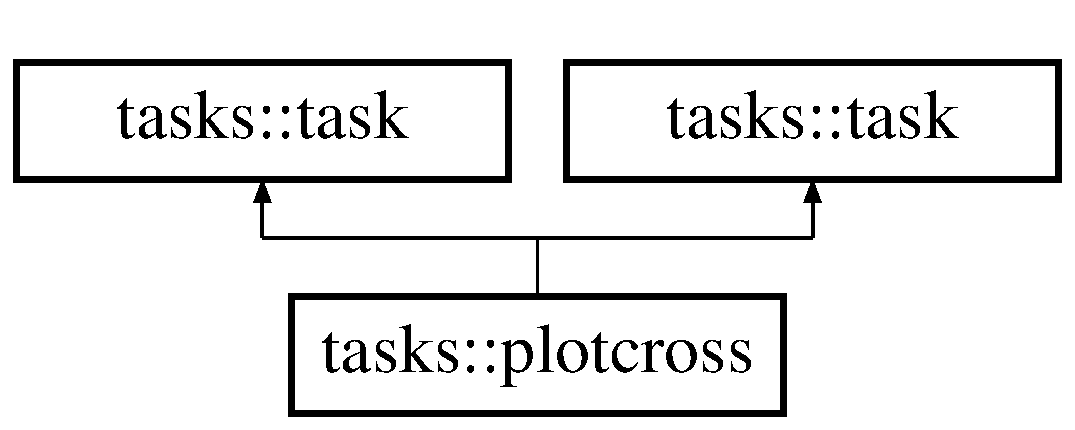
\includegraphics[height=2cm]{classtasks_1_1plotcross}
\end{center}
\end{figure}
\subsection*{Public Member Functions}
\begin{CompactItemize}
\item 
def \textbf{run}\label{classtasks_1_1plotcross_0a8e5cdcfe67c0318ca5c81ad986491c}

\item 
def \textbf{run}\label{classtasks_1_1plotcross_0a8e5cdcfe67c0318ca5c81ad986491c}

\end{CompactItemize}
\subsection*{Static Public Attributes}
\begin{CompactItemize}
\item 
string \textbf{name} = '{\bfplotcross}'\label{classtasks_1_1plotcross_bd7609b129ee55f318dea09cf1977257}

\item 
string \textbf{button\-Text} = 'Plot cross-order profile'\label{classtasks_1_1plotcross_ee5e9fdfa52617ca2fbd39736885b86e}

\item 
list \textbf{prereq} = ['{\bfpreproc}']\label{classtasks_1_1plotcross_467eea84daabfbe4a8772e98a68bb74f}

\item 
int \textbf{output} = 0\label{classtasks_1_1plotcross_830ab0e671403732f95073f3113b7c77}

\end{CompactItemize}


\subsection{Detailed Description}


\footnotesize\begin{verbatim}Plot the cross-order profile. The profile is an average of the central 5
   columns of the frame.
\end{verbatim}
\normalsize
 



The documentation for this class was generated from the following files:\begin{CompactItemize}
\item 
old/PANICtool-1.0/tasks.py\item 
old/tasks.py\end{CompactItemize}
